\chapter{Methodology}
\label{chap:methodology}

\section{Developement of the simulation model}

\subsection{Specifications}
\label{sub:spec}
In order to use the use the characterisitc equation of hydroelectricity (eq. \ref{eq_power_2} page \pageref{eq_power_2}) and predict with precision the electrical output of a run-of-the-river power plant, the following parameters and values would be needed : 
\begin{itemize}
\itemsep0em
 \item Power plant parameters : 
 \begin{itemize}
  \item nominal water flow through the turbine ($\dot{V}_\mathrm{n}$)
  \item nominal head of water ($h_\mathrm{n}$)
  \item nominal water level ($W_\mathrm{n}$)
  \item efficiency curve of the turbine ($\eta_\mathrm{turbine}$) 
  \item efficiency of the generator ($\eta_\mathrm{generator}$)  
  \item unusable water flow ($\dot{V}_\mathrm{rest}$)  
 \end{itemize}
 \item Input time series : 
 \begin{itemize}
  \item actual water flow through the turbine ($\dot{V}$)
  \item actual water level downstream from the turbine ($W$)
 \end{itemize}
\end{itemize}

However, if such precise data can be found for single power plants, it is not easily accessible at a state or country-wide level. The OEDB database lists the location and nominal power of the plants, without further information on their design. The german Bundesnetzagentur is developing a register of every energy production facility in Germany, called ``Marktstammdatenregister''. This register should give a complete overview of the power plants in Germany, sorted by energy carrier and type of plant (reservoir, run-of-the-river, pumped hydro...), and listing the location and nominal power, as well as the presence or not of a restriction of the usable water flow due to a fish ladder or fish protection system for instance \cite{MaStR}. This last information is not yet available in registers such as the OEDB.\newline
Therefore, the model should be able to extrapolate missing data and to make some assumptions when optional input parameters are not provided. The only compulsory input parameter will be the broadly available nominal power of the turbine and subsections \ref{sub:assumptions} and \ref{sub:extrapolation} explains how other parameters can be assumed or extrapolated. \newline
In terms of time series, in addition to the water flow over the simulated period, the model will take as input the water flow over several years in order to extrapolate missing parameters.\\
The desired outputs for the model are electricity production time series per power plant or per area. It should also be possible to simulate several plants in one go.

\subsection{Assumptions}
\label{sub:assumptions}
In order to simplify the model, some assumptions were made regarding parameters whose variations have a limited impact on the end results. \\
The first assumption regards the efficiency of the generator. Section \ref{sub:gen_eff} detailled how the generator efficiency is dependant on its power and part-load range. It is estimated that among the 6500 to 7500 hydropower plants in Germany, only 406 have a nominal power above \unit[1]{MW} \cite{uba_wasserkraft}. Out of 7500 run-of-the-river hydropower plants in the OpenEnergy Database, 5600 have a capacity under 100kW (see figure \ref{oedb_capa} page \pageref{hpp_register}). However, the plants under \unit[1]{MW} (and therefore to a bigger extent the plants under \unit[100k]{W}) account for a small part of the total installed power (see figure \ref{uba_hpp}). For that reason, the generator efficiency has been approximated to \unit[95]{\%} for all power plants is this work. XXX maybe include variable gen efficiency in model and delete this XXX

\begin{figure}[H]
\centering
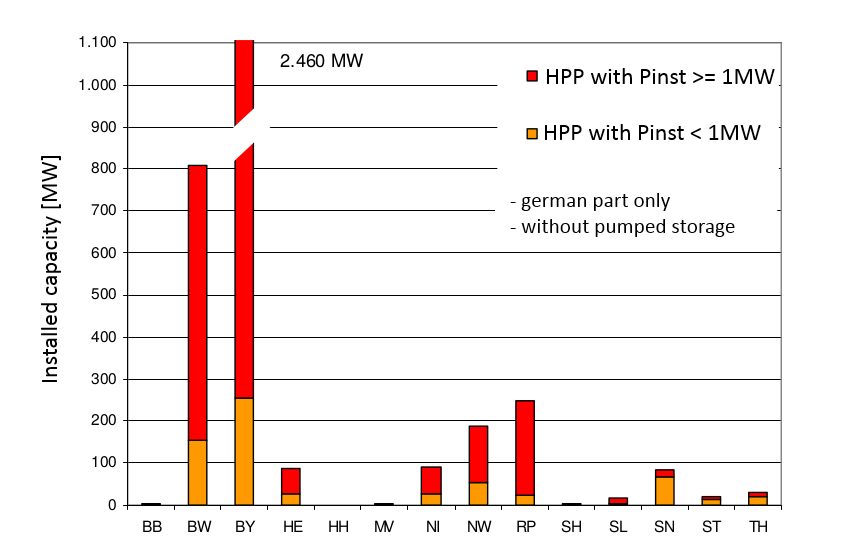
\includegraphics[width=15cm]{uba_hpp_en.png}
\caption[Installed power pro Bundesland for plants over and under {\unit[1]{MW}}]{Installed power pro Bundesland for plants over and under {\unit[1]{MW}} \cite{uba_wasserkraft}}
\label{uba_hpp}
\end{figure}

The second assumption regards the variability of the head of water. The equation \ref{eq_head} given on page \pageref{eq_head} gives the relation between the head and the water level. Section \ref{meas_runoff} shows that measured data for water level is widely available throughout Germany, however this data is only valid on the site of the gauge. Figures \ref{mosel_WQ} based on measurement data for three stations on the Mosel from the Deutsches Gewässerkundliches Jahrbuch show that water level and water flow have a linear correlation, and figure \ref{Q_mosel} (see appendix \ref{app:boxplot} on how to read the graph) shows that the water flow augments gradually as tributaries merge with the river. However, the water level does not depend on the distance to the river mouth (see fig. \ref{W_mosel} and appendix \ref{app:boxplot}). This is due to the fact that the correlation factor between water flow and water level depends on the shape of the river bed. This strong variability of water level from a place to another would biase the results if the equation \ref{eq_head} (p.\pageref{eq_head}) was used. For that reason, the model will approximate the head of water $h$ with the nominal head $h_\mathrm{n}$.

\begin{figure}[H]
\centering
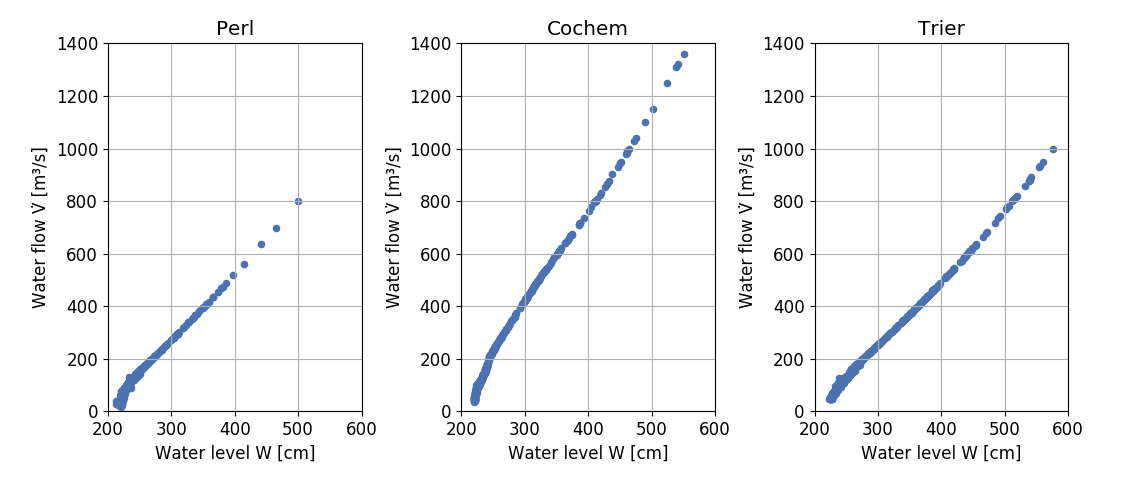
\includegraphics[width=15cm]{mosel_WQ.png}
\caption[Linear correlation between W and  \.{V} for three places on the Mosel]{Linear correlation between W and  \.{V} for three places on the Mosel}
\label{mosel_WQ}
\end{figure}

\begin{figure}[H]
\centering
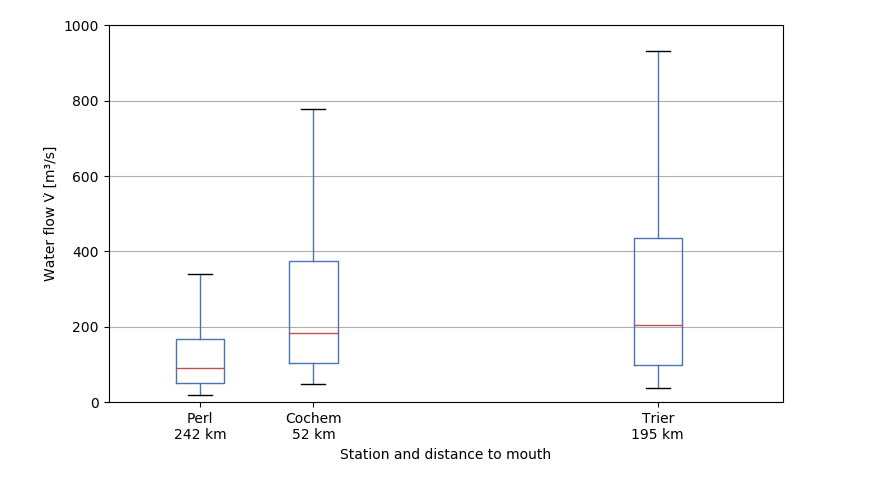
\includegraphics[width=15cm]{Q_mosel.png}
\caption[Distribution of water flow for three places on the Mosel]{Distribution of water flow for three places on the Mosel}
\label{Q_mosel}
\end{figure}

\begin{figure}[H]
\centering
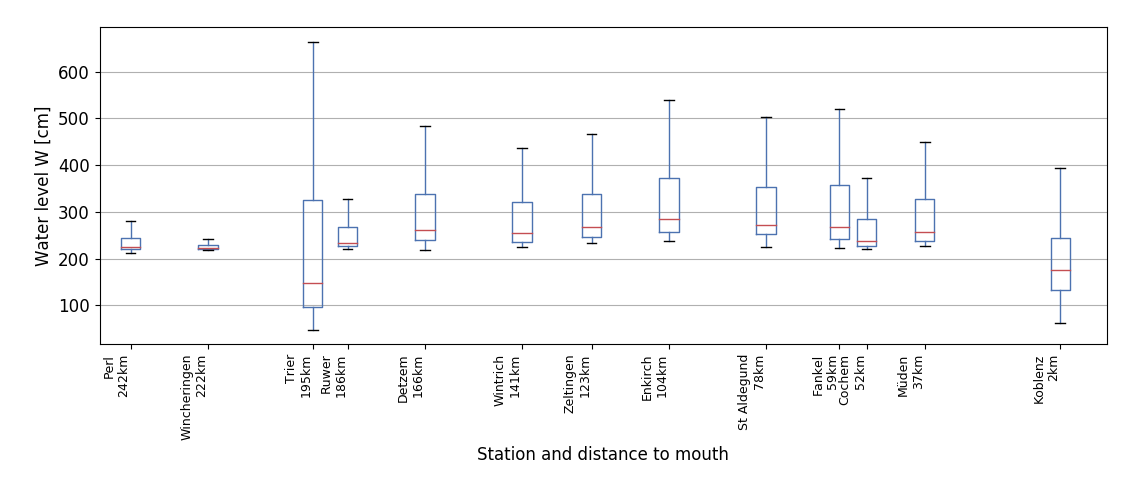
\includegraphics[width=15cm]{W_mosel.png}
\caption[Distribution of water level at gauges on the Mosel]{Distribution of water level at gauges on the Mosel}
\label{W_mosel}
\end{figure}

\subsection{Extrapolation}
\label{sub:extrapolation}
A specification of the model, as explained in subsection \ref{sub:spec}, is to be able to run the simulation with limited information about the power plant, namely the nominal power and the coordinates. To do so, the other necessary information (nominal head, nominal inflow, and type of turbine) will be extrapolated from the hydrological history of the location, following the steps of the design process for a run-of-the-river plant.\\
The first step is to decide of the nominal inflow of the turbine. This is done by examining the history of water flow of the location over several years and taking into account the residual water quantity required by law.
The residual water quantity is regulated by law, and therefore depends on the country, or on the federal state in Germany. Giesecke gives several ways of defining the residual water quantity and shows that they give slightly differents values \cite{gies_qrest}. In this work, a formula-based approach was used to calculate the residual water (see tab. \ref{res_wat}), where \.{V}\textsubscript{347} is the water flow that 347 days a year reached or exceeded is, averaged over 10 years. 
\begin{table}
 \centering
 \caption[Residual water quantity depending on the river]{Residual water quantity depending on the river \cite{gies_qrest}}
 \label{res_wat}
 \begin{tabular}{|l|c|}
  \hline
  \multicolumn{1}{|c|}{\.{V}\textsubscript{347}} & \.{V}\textsubscript{rest}\\
  \hline
  Up to \unit[60]{l\textperiodcentered s\textsuperscript{-1}}&\unit[50]{l\textperiodcentered s\textsuperscript{-1}}\\
  And for each further \unit[10]{l\textperiodcentered s\textsuperscript{-1}} & \unit[10]{l\textperiodcentered s\textsuperscript{-1}} more\\
  \hline
  For \unit[160]{l\textperiodcentered s\textsuperscript{-1}}&\unit[130]{l\textperiodcentered s\textsuperscript{-1}}\\
  And for each further \unit[10]{l\textperiodcentered s\textsuperscript{-1}} & \unit[4.4]{l\textperiodcentered s\textsuperscript{-1}} more\\
  \hline
  For \unit[500]{l\textperiodcentered s\textsuperscript{-1}}&\unit[280]{l\textperiodcentered s\textsuperscript{-1}}\\
  And for each further \unit[100]{l\textperiodcentered s\textsuperscript{-1}} & \unit[31]{l\textperiodcentered s\textsuperscript{-1}} more\\  
  \hline
  For \unit[2500]{l\textperiodcentered s\textsuperscript{-1}}&\unit[900]{l\textperiodcentered s\textsuperscript{-1}}\\
  And for each further \unit[100]{l\textperiodcentered s\textsuperscript{-1}} & \unit[21.3]{l\textperiodcentered s\textsuperscript{-1}} more\\  
  \hline
  For \unit[10000]{l\textperiodcentered s\textsuperscript{-1}}&\unit[2500]{l\textperiodcentered s\textsuperscript{-1}}\\
  And for each further \unit[1000]{l\textperiodcentered s\textsuperscript{-1}} & \unit[150]{l\textperiodcentered s\textsuperscript{-1}} more\\  
  \hline
  From \unit[60000]{l\textperiodcentered s\textsuperscript{-1}}&\unit[10000]{l\textperiodcentered s\textsuperscript{-1}}\\
  \hline
 \end{tabular}
\end{table}
The nominal water flow is chosen so that the power plant works at full load a given number of days a year. The literature recommends that the nominal water flow should be reached 50 to 90 days a year for a system connected to the grid, or 250 days a year for an isolated operation (self-production) \cite{pacer}\cite{cetmef}. The value of 120 days (30\% of the year) can also be found \cite{cetmef}. The nominal water flow is obtained by analyzing the flow duration curve over as many years as possible. This work will use the value of 70 days a year. However, this can lead to errors, as the real value is influenced by economical and human factors.\\
Even though the potential head of water could be calculated from the altitude variations along the river, it would be difficult to access what technically and economically feasible is, without precise information on the location. However, the nominal head can be easily calculated from the nominal water flow and the nominal power, using equation \ref{head_calc}. At this point of the process, the type of turbine is not known. However, figure \ref{efficiency_turb} page \pageref{efficiency_turb} shows that at full load, all types of turbines have an efficiency around 90\%.

\begin{equation}
\label{head_calc} 
 h = \frac{P_\mathrm{n}}{\rho_\mathrm{water} \cdot g \cdot \dot{V}_\mathrm{n} \cdot \eta_\mathrm{turbine,n} \cdot \eta_\mathrm{generator,n}}
\end{equation}

Finally, the type of turbine is set using a characteristic diagram (fig. \ref{charac_diag}). 

\begin{figure}[H]
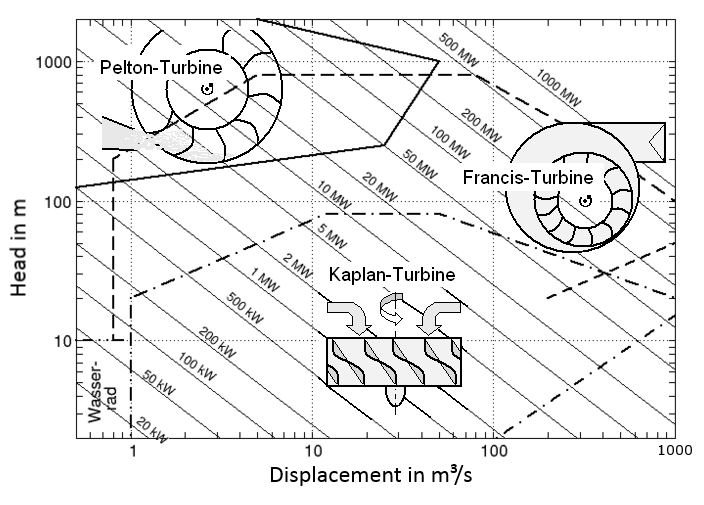
\includegraphics[width=14cm]{charac_diag_en.png}
\caption[Characteristic diagram for several types of water turbines]{Characteristic diagram for several types of water turbines \cite{wiki_WK}}
\centering
\label{charac_diag}
\end{figure}

\subsection{Collection and administration of data basis}

Considering the assumptions made in the previous subsection (sec. \ref{sub:assumptions}), the list of necessary data from subsection \ref{sub:spec} becomes :
\begin{itemize}
 \item Water flow data (time series for the period to simulate)
 \item Geographical data (river courses)
 \item Properties of installed run-of-the-river power plants :
 \begin{itemize}
  \item Coordinates
  \item Installed capacity
  \item Nominal head or nominal inflow or history of water flows
  \item Type of turbine or characteristic diagramm of turbines
 \end{itemize}
 \item Real production data for validation
\end{itemize}

This data has to be collected and pre-processed to serve as input for the model.

\subsection{Simulation results and evaluation}


For this reason, the state-wide simulation of hydropower production presented in the case study from section XXX UPDATE WHEN READY XXX as been conducted for XXX TH or ST or MV XXX, in order to compare the results of the simulation based on the OEDB register with the yearly production values given by the AEE.

In this work, data from the BfG was used as input to test the model (XXX put references of teil über Mosel und Thuringe XXX), as well as data from the french ``Banque Hydro'' (XXX reference of the teil über Hydroraon XXX). The ``Banque Hydro'' is run by the SCHAPI (Service Central d'Hydrométéorologie et d'Appui à la Prévision des Inondations), a section of the french Ministry of Ecology, Sustainable Development and Energy, and gathers data from around 5000 gauge stations.


XXX Over which period of time, stepsize, error...

\section{Data preprocessing}

\subsection{Power plants register - OEDB}
XXX GIS/SQL code from Ludwig. Next neighbour finden, gauge station has to be on the same river...
\subsection{Runoff data}
XXX structure in DB

\section{Simulation}

\section{Evaluation of results}

